% !TeX program = pdflatex
\documentclass[tikz,border=8pt]{standalone}
\usepackage{pgfplots}\pgfplotsset{compat=1.16}
\definecolor{FigureOrange}{HTML}{EA580C}
\begin{document}
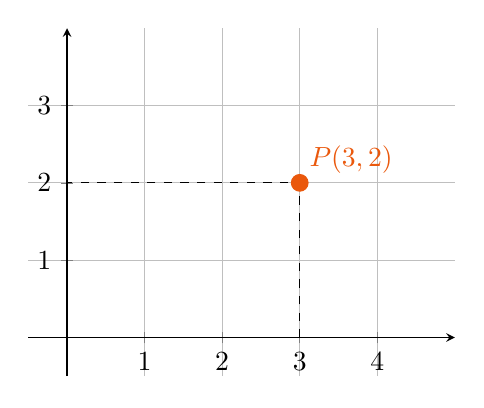
\begin{tikzpicture}
\begin{axis}[width=7cm,height=6cm,axis lines=middle,xmin=-.5,xmax=5,ymin=-.5,ymax=4,xtick={0,1,2,3,4},ytick={0,1,2,3},grid=both,clip=false]
  \addplot[only marks,mark=*,mark size=3pt,FigureOrange] coordinates {(3,2)};
  \draw[dashed] (axis cs:3,0)--(axis cs:3,2)--(axis cs:0,2);
  \node[above right,FigureOrange] at (axis cs:3,2) {$P(3,2)$};
\end{axis}
\end{tikzpicture}
\end{document}
